%----------------------------------------------------------------------
%	DIRC TECHNOLOGY CHAPTER
%----------------------------------------------------------------------
\label{ch:dirc}
DIRC detectors are based on the concept of the Detection of Internally Reflected Cherenkov light (DIRC) produced in a solid radiator bar to identify charged particle. It is a special type of Cherenkov counter, which uses the unique properties of Cherenkov radiation to identify charged particle species.

%----------------------------------------------------------------------
%	CHERENKOV RADIATION SECTION
%----------------------------------------------------------------------
\section{Cherenkov Radiation}
Einstein postulated in his Theory of Relativity that the speed of light in a vacuum, $c$, is the limit of the velocity of massive particles. In an optically transparent medium, however, the speed at which light propagates is modified: $c_{med} = c/n$, where $n$ is the index of refraction of the medium. Pavel Cherenkov discovered in 1934 that massive particles moving through a medium faster than the speed of light in that medium emit light in the form of now-called Cherenkov radiation. Cherenkov was able to establish several interesting properties of this radiation: it is only emitted from charged particles above a certain velocity threshold $v > c/n$, the intensity is proportional to the particle's path length, emission is prompt, and the light is polarized with a continuous wavelength spectrum. Later in 1937 Ilya Frank and Igor Tamm theoretically formulated this radiation with fantastic agreement to Cherenkov's findings, and the three shared the 1958 Nobel Prize in Physics for their efforts \cite{CherenkovHistory}.

Further studies confirmed that Cherenkov radiation is emitted uniformly in azimuth ($\phi_c$) around the particle's direction of travel with the polar opening angle $\thetaC$ defined as

\begin{equation}
	\cos\thetaC = \frac{1}{\beta n(\lambda)},
	\label{eq:cherenkovformula}
\end{equation}

where $\beta = v_p/c$, $v_p$ is the particle's velocity, and the index of refraction is a function of the emitted photon wavelength. In a normal, dispersive optical medium the opening half-angle of the shock wave produced by the Cherenkov radiation, $\eta_C$ defined in Figure \ref{fig:cherenkovcone}, is not complementary to the Cherenkov angle. The relationship between the two is given by

\begin{equation}
	\cot\eta_C = \left[\frac{\diff}{\diff\omega}(\omega \tan\thetaC) \right]_{\omega_0} = \left[\tan\thetaC + \beta^2\omega n(\omega) \frac{\diff n}{\diff\omega}\cot\thetaC \right]_{\omega_0}
	\label{eq:openingangle}
\end{equation}
where $\omega_0$ is the central vale of the considered frequency range. Because the second term in (\ref{eq:openingangle}) is zero only for non-dispersive media the shock wave front is not perpendicular to the Cherenkov cone in real detectors.

\begin{figure}[!htb]
	\centering
	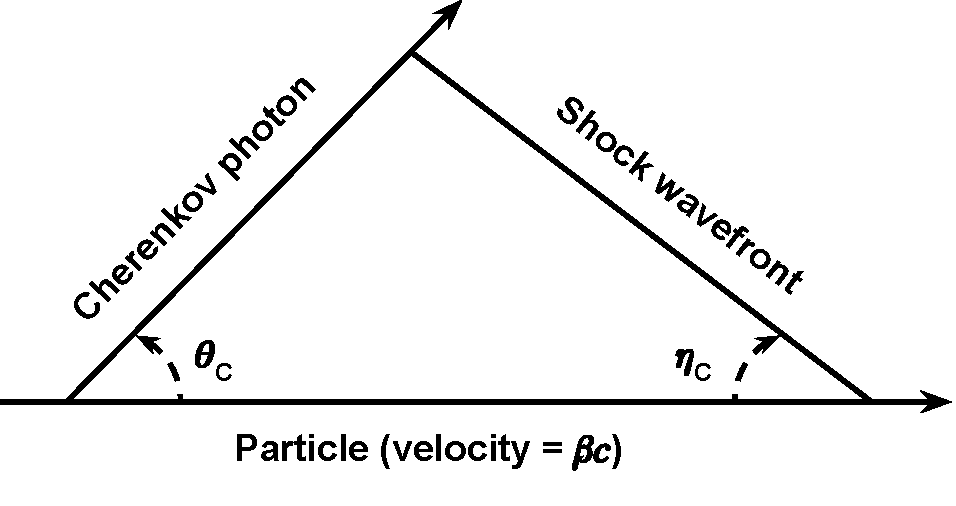
\includegraphics[scale=1]{Cherenkov_cone.pdf}
	\caption{Illustration of the Cherenkov cone.}
	\label{fig:cherenkovcone}
\end{figure}

Because particles lose very little energy when radiating Cherenkov photons the emission is very weak. The number of photons $N_{photons}$ emitted per path length $L$ (in cm) by a moving particle with charge $z$ is given by the Frank-Tamm equation

\begin{equation}
	\frac{N_{photons}}{L} = \frac{\alpha^2 z^2}{r_e m_e c^2} \int \sin^2\thetaC (E) \diff E
	\label{eq:nphotons}
\end{equation}
where E is the photon energy in eV, the integral is taken over the region where $n(E)$ is greater than 1, $\alpha = \frac{1}{137}$ is the fine structure constant, $z$ is the projective charge in units of electron charge, and $\frac{\alpha^2 z^2}{r_e m_e c^2} = 370\unit{cm}^{-1}\unit{eV}^{-1}$.

%----------------------------------------------------------------------
%	APPLYING TO PID SECTION
%----------------------------------------------------------------------
\section{Applying the Cherenkov Effect to Particle ID}
In order to identify particle species one must know both the mass and charge of the particle in question. Because the Cherenkov angle encodes the particle's velocity it is, in principle, a simple matter to measure the particle's momentum with a tracking chamber as well as the velocity obtained from (\ref{eq:cherenkovformula}) to determine the mass and charge. Figure \ref{fig:angleseperation} shows how different particle species can be distinguished for a given momentum in fused silica.

Threshold counters are Cherenkov detectors used for particle identification (PID) by exploiting the fact that only particles above the threshold velocity $\beta > 1/n$ will emit Cherenkov photons. Therefore lighter particles will emit Cherenkov light while heavier particles will not for a given momentum. The information about a particle's velocity can be combined with momentum information from a tracking system to determine the mass as \cite{ParticleDetectionHandbook}

\begin{equation}
	m = \frac{p}{c} \sqrt{n^2 \cos^2\thetaC - 1}
	\label{eq:mass}
\end{equation}

\begin{figure}[!htb]
	\centering
	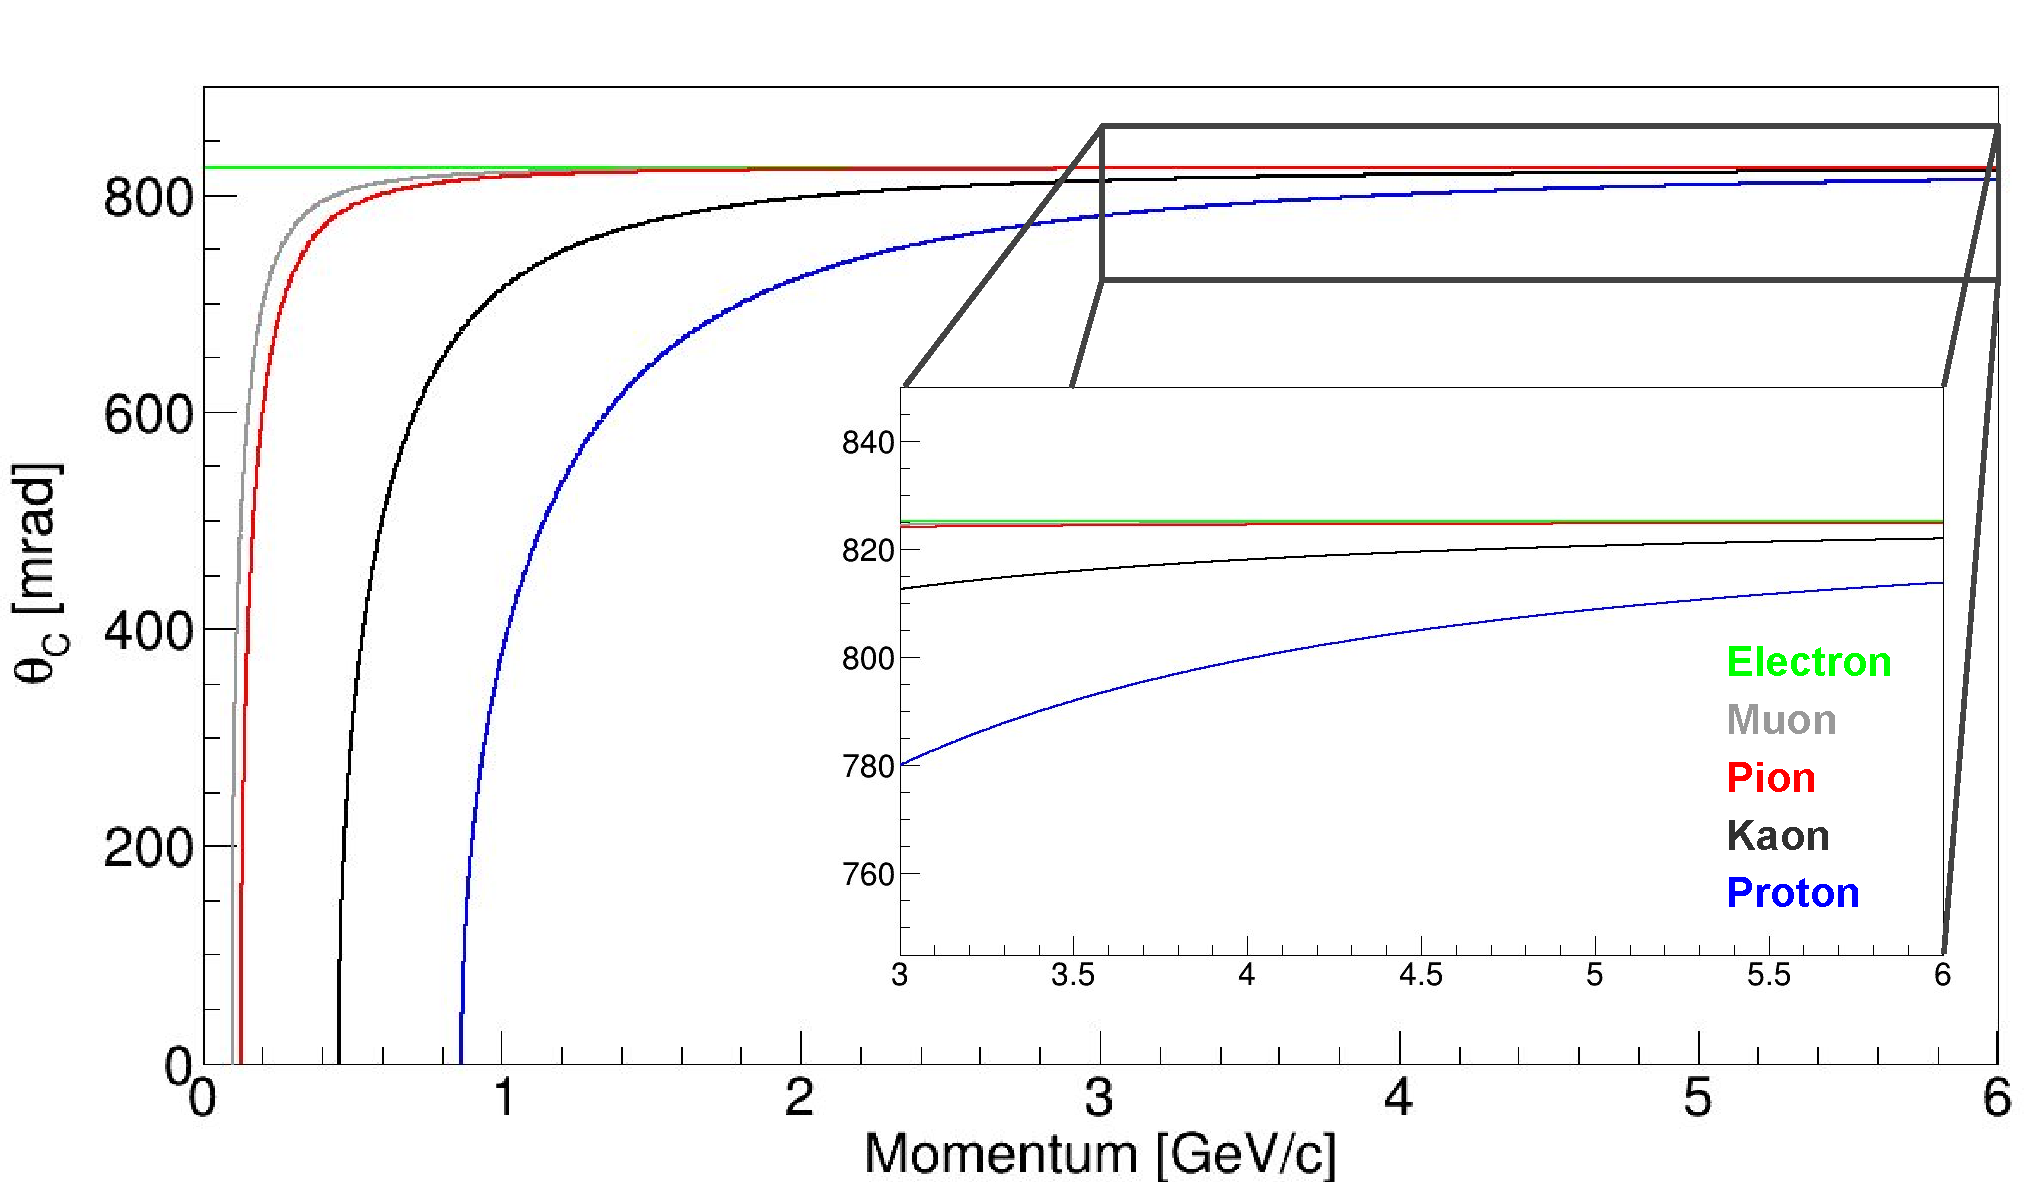
\includegraphics[width=\textwidth]{angle_seperation_enhance.pdf}
	\caption{Particle momentum [GeV/c] versus Cherenkov angle [mrad] for different particle species in fused silica ($n \approx 1.473$). While the full range (left) makes it seem as if separation between heavier species becomes more and more challenging, zooming in (right) shows that it is indeed possible separate protons, kaons, and pions even at higher particle momentum.}
	\label{fig:angleseperation}
\end{figure}

%----------------------------------------------------------------------
%	RICH SECTION
%----------------------------------------------------------------------
\section{Ring Imaging Detectors}
Ring Imaging Cherenkov (RICH) detectors are designed to efficiently identify and separate different particle species over a wide range of momenta. A basic RICH system is shown in Figure \ref{fig:rich_basics}. 

\begin{figure}[!htb]
	\centering
	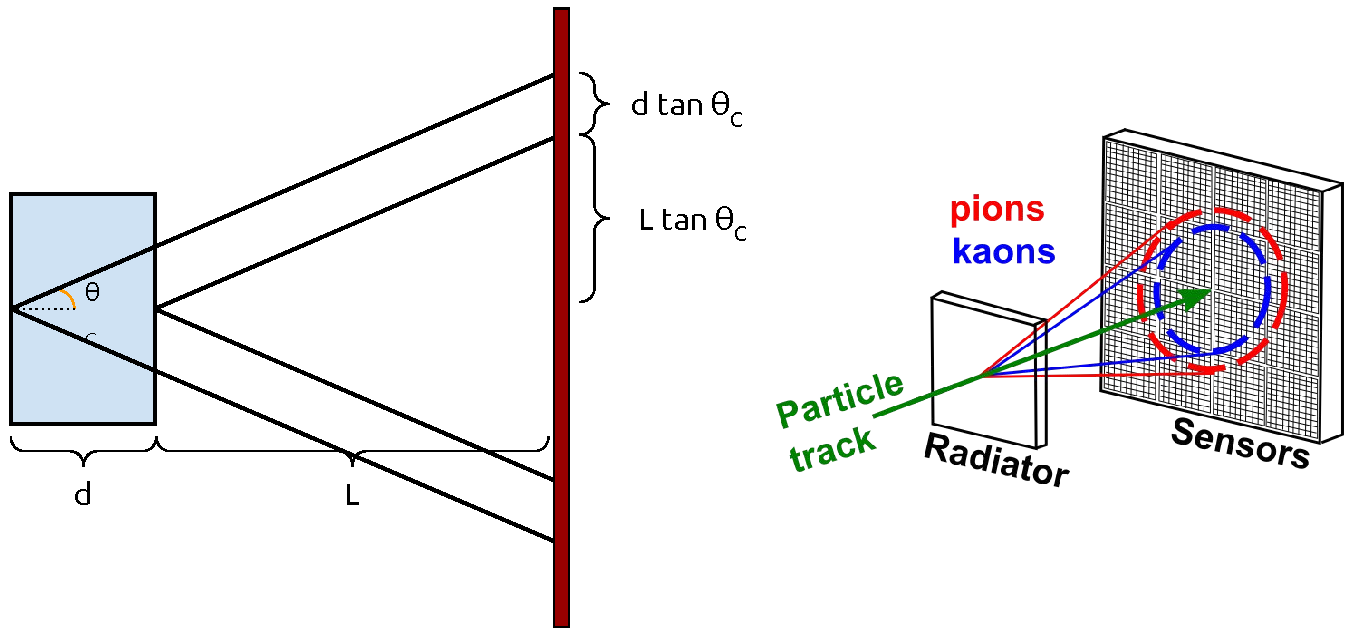
\includegraphics[width=\textwidth]{RICH_rings.pdf}
	\caption{Basic concept of a proximity focusing Ring Imaging Cherenkov (RICH) detector (a), and an example of how they can be used to do PID based on particle mass (b).}
	\label{fig:rich_basics}
\end{figure}

A volume of radiator, either gaseous (e.g. $C_{4}F_{10}$) or solid (e.g. aerogel), is positioned upstream of an array of photosensors. A charged particle traveling through a thin radiator above the threshold velocity will continuously emit Cherenkov photons in a cone. The resulting image on the photosensor array is an annulus of thickness $d\tan\thetaC$ and an inner radius of $L\tan\thetaC$, where $d$ is the distance the particle traveled inside the radiator, $L$ is the distance between the radiator and the photosensors, and  $\thetaC$ is the usual Cherenkov angle (Figure \ref{fig:rich_basics}b). PID is done by measuring the average radius of the annulus and reconstructing the Cherenkov angle geometrically.


%----------------------------------------------------------------------
%	DIRC SECTION
%----------------------------------------------------------------------
\section{DIRC Detectors}
DIRC detectors work much the same way as a RICH in that they collect Cherenkov photons produced from a radiating material and use the created image on the photosensors to reconstruct the Cherenkov angle. In the case of a DIRC, the radiating medium is also used as a light guide as some of the Cherenkov photons undergo total internal reflection inside the radiator and are guided towards one end of the radiator to a readout (Figure \ref{fig:dircbasics}). The radiator of choice is a solid bar made of fused silica, with an index of refraction $n \approx 1.473$. A rectangular cross section and highly smoothed and polished sides ensure that the magnitude of the Cherenkov angle is preserved during internal reflection. Photons that are created propagating away from the readout are reflected back towards the readout by a mirror. Once the photons exit the radiator they are allowed to separate through an expansion volume before being imaged in both ($x, y$) position as well as time. The arrival position and propagation time of each detected photon are combined with tracking information to reconstruct the Cherenkov angle and determine the corresponding PID likelihoods (reconstruction methods and techniques for DIRC detectors will be discussed in detail in Chapter \ref{ch:analysis}).

\begin{figure}[!htb]
	\centering
	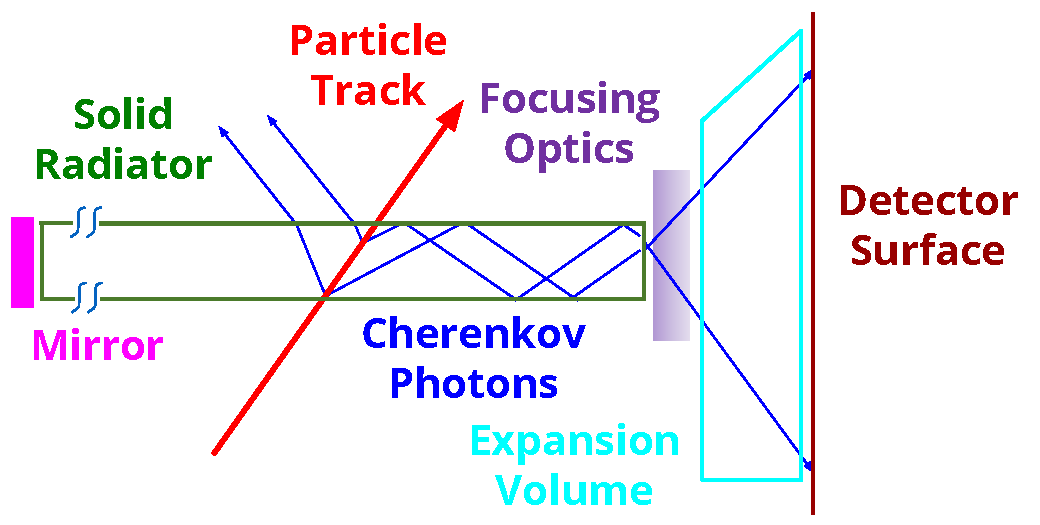
\includegraphics[scale=0.7]{DIRC_components.pdf}
	\caption{The basic components of a DIRC detector: a solid radiator, typically fused silica (green); a mirror to redirect backward-going photons (pink); optional focusing optics (purple); an expansion volume to allow photons to separate in space (cyan); and a detector surface to record the position and arrival time of Cherenkov photons (blue).}
	\label{fig:dircbasics}
\end{figure}

The performance of a DIRC detector is given by the resolution in the Cherenkov polar opening angle of the particle track, $\sigma_{\thetaC,\text{track}}^2$, which can be written as:

\begin{equation}
	\sigma_{\thetaC,\text{track}}^2 = \sigma_{\thetaC}^2 / N_{\gamma} + \sigma_{\text{correlated}}^2
	\label{eq:performance}
\end{equation}

where $\sigma_{\thetaC}$ is the average single photon Cherenkov angle resolution, $N_{\gamma}$ is the number of measured photons per track, and $\sigma_{\text{correlated}}$ includes several correlated terms that contribute to the resolution such as the uncertainty in the particle track direction coming from external tracking systems. Because the track direction is crucial to the reconstruction of the Cherenkov angle, this error needs to be small for the performance to not suffer. For the EIC a tracking resolution on the order of 1 mrad is required for adequate PID.

\begin{figure}[!htb]
	\centering
	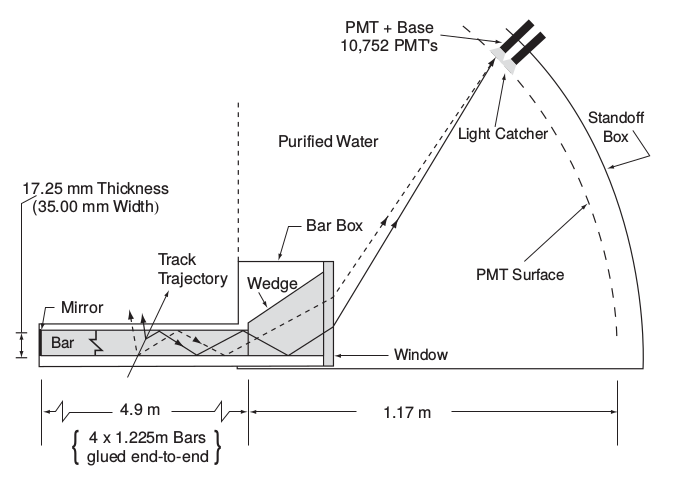
\includegraphics[width=\textwidth]{BaBar_DIRC.png}
	\caption{Schematic of BaBar DIRC and detection region.}
	\label{fig:babardirc}
\end{figure}

As of the writing of this thesis the only DIRC detector used in a full experiment is the BaBar DIRC at SLAC National Accelerator Laboratory, which was successfully operated from 1999 through 2008 \cite{BaBarDIRC}. It proved to be a robust, stable, and easy to operate system for more than 8 years, providing excellent pion/kaon separation for all tracks from $B$-meson decays. It used 4.9 m long radiator bars with a rectangular cross section of $17.25 \times 35 \unit{mm}^2$. Each bar was made of four $1.225\unit{m}$ long fused silica bars glued end-to-end. The bars were placed in 12 hermetically sealed containers, called bar boxes, each holding 12 radiator bars for a total of 144 bars. At the end of each box was attached a wedge of fused silica and a window to allow the photons to expand before entering the water-filled expansion volume and being read out on one of 10,752 photomultiplier tubes (see Figure \ref{fig:babardirc}). Figure \ref{fig:babarperformance} summarizes the performance of the BaBar DIRC, showing excellent Cherenkov angle reconstruction (2.5 mrad, only 14\% larger than the design goal of 2.2 mrad) and photon yield per track.

\begin{figure}[!htb]
	\centering
	a)%
	\raisebox{-1.0\height}{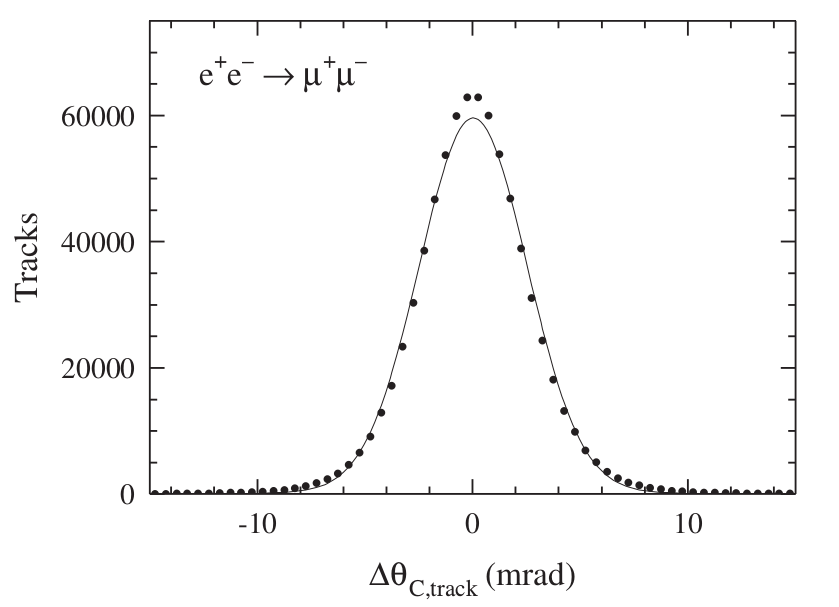
\includegraphics[width=0.5\textwidth]{BaBar_SPR.png}}%
	b)%
	\raisebox{-1.0\height}{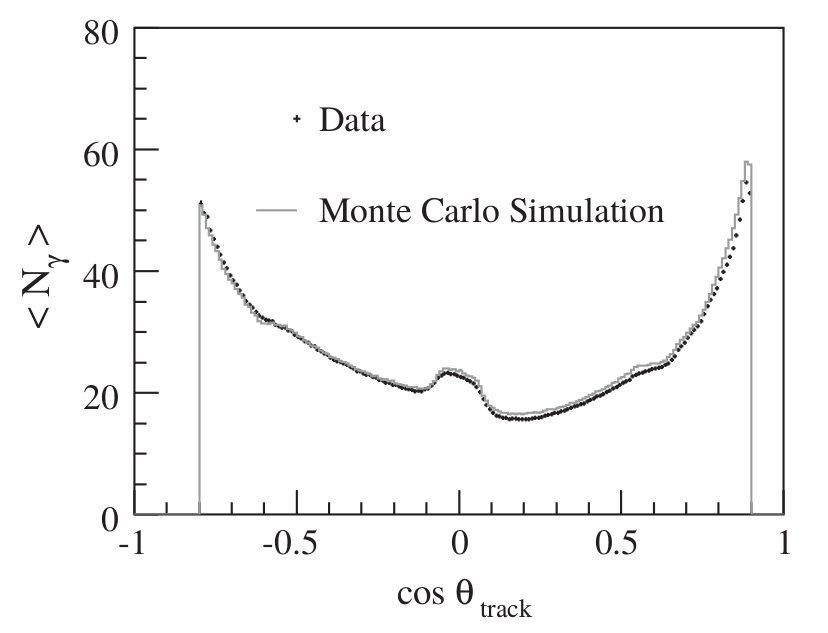
\includegraphics[width=0.5\textwidth]{BaBar_NPH.png}}
	\caption{Performance of the BaBar DIRC for $e^{+}e^{-} \rightarrow \mu^{+}\mu^{-}$ events. a) shows the difference between the measured and expected Cherenkov angle (dots) and a Gaussian fit to the data with a 2.5 mrad width (line). b) is the average number of detected photons vs. track polar angle for data (dots) and Geant4 \cite{Geant4} simulation (line).}
	\label{fig:babarperformance}
\end{figure}

\subsection{DIRCs in Future Experiments}
The BaBar DIRC has since inspired many other experiments/facilities, including the EIC, to utilize this new, novel PID system in a variety of ways (Figure \ref{fig:dirc_evolution}). The Focusing DIRC (FDIRC) proposed for the now-cancelled SuperB collider in Italy was the first to propose using some form of focusing for the Cherenkov photons, allowing for a factor of 10 smaller expansion volume \cite{FDIRC}. The barrel DIRC for the PANDA experiment at FAIR in Germany will use shorter radiator bars for a more compact design \cite{PANDA_barrel}, while the PANDA disc DIRC will be used in the forward region and will be the first disc DIRC to be used in a high-performance $4\pi$ detector \cite{PANDA_disc}. Belle II at the SuperKEKB accelerator in Japan will utilize wide plates as radiators and focus on fast timing for PID in the barrel region \cite{Belle2_TOP}. The TORCH detector, similar to the PANDA disc DIRC, will be a large-area detector focusing on precision time-of-flight to do PID for low momentum kaons at the upgraded LHCb experiment \cite{TORCH}. The GlueX experiment at JLab will be recycling four bar boxes from the BaBar experiment to cover the forward region of their spectrometer; utilizing  focusing similar to the FDIRC design \cite{GlueX}.

\begin{figure}[H]
	\centering
	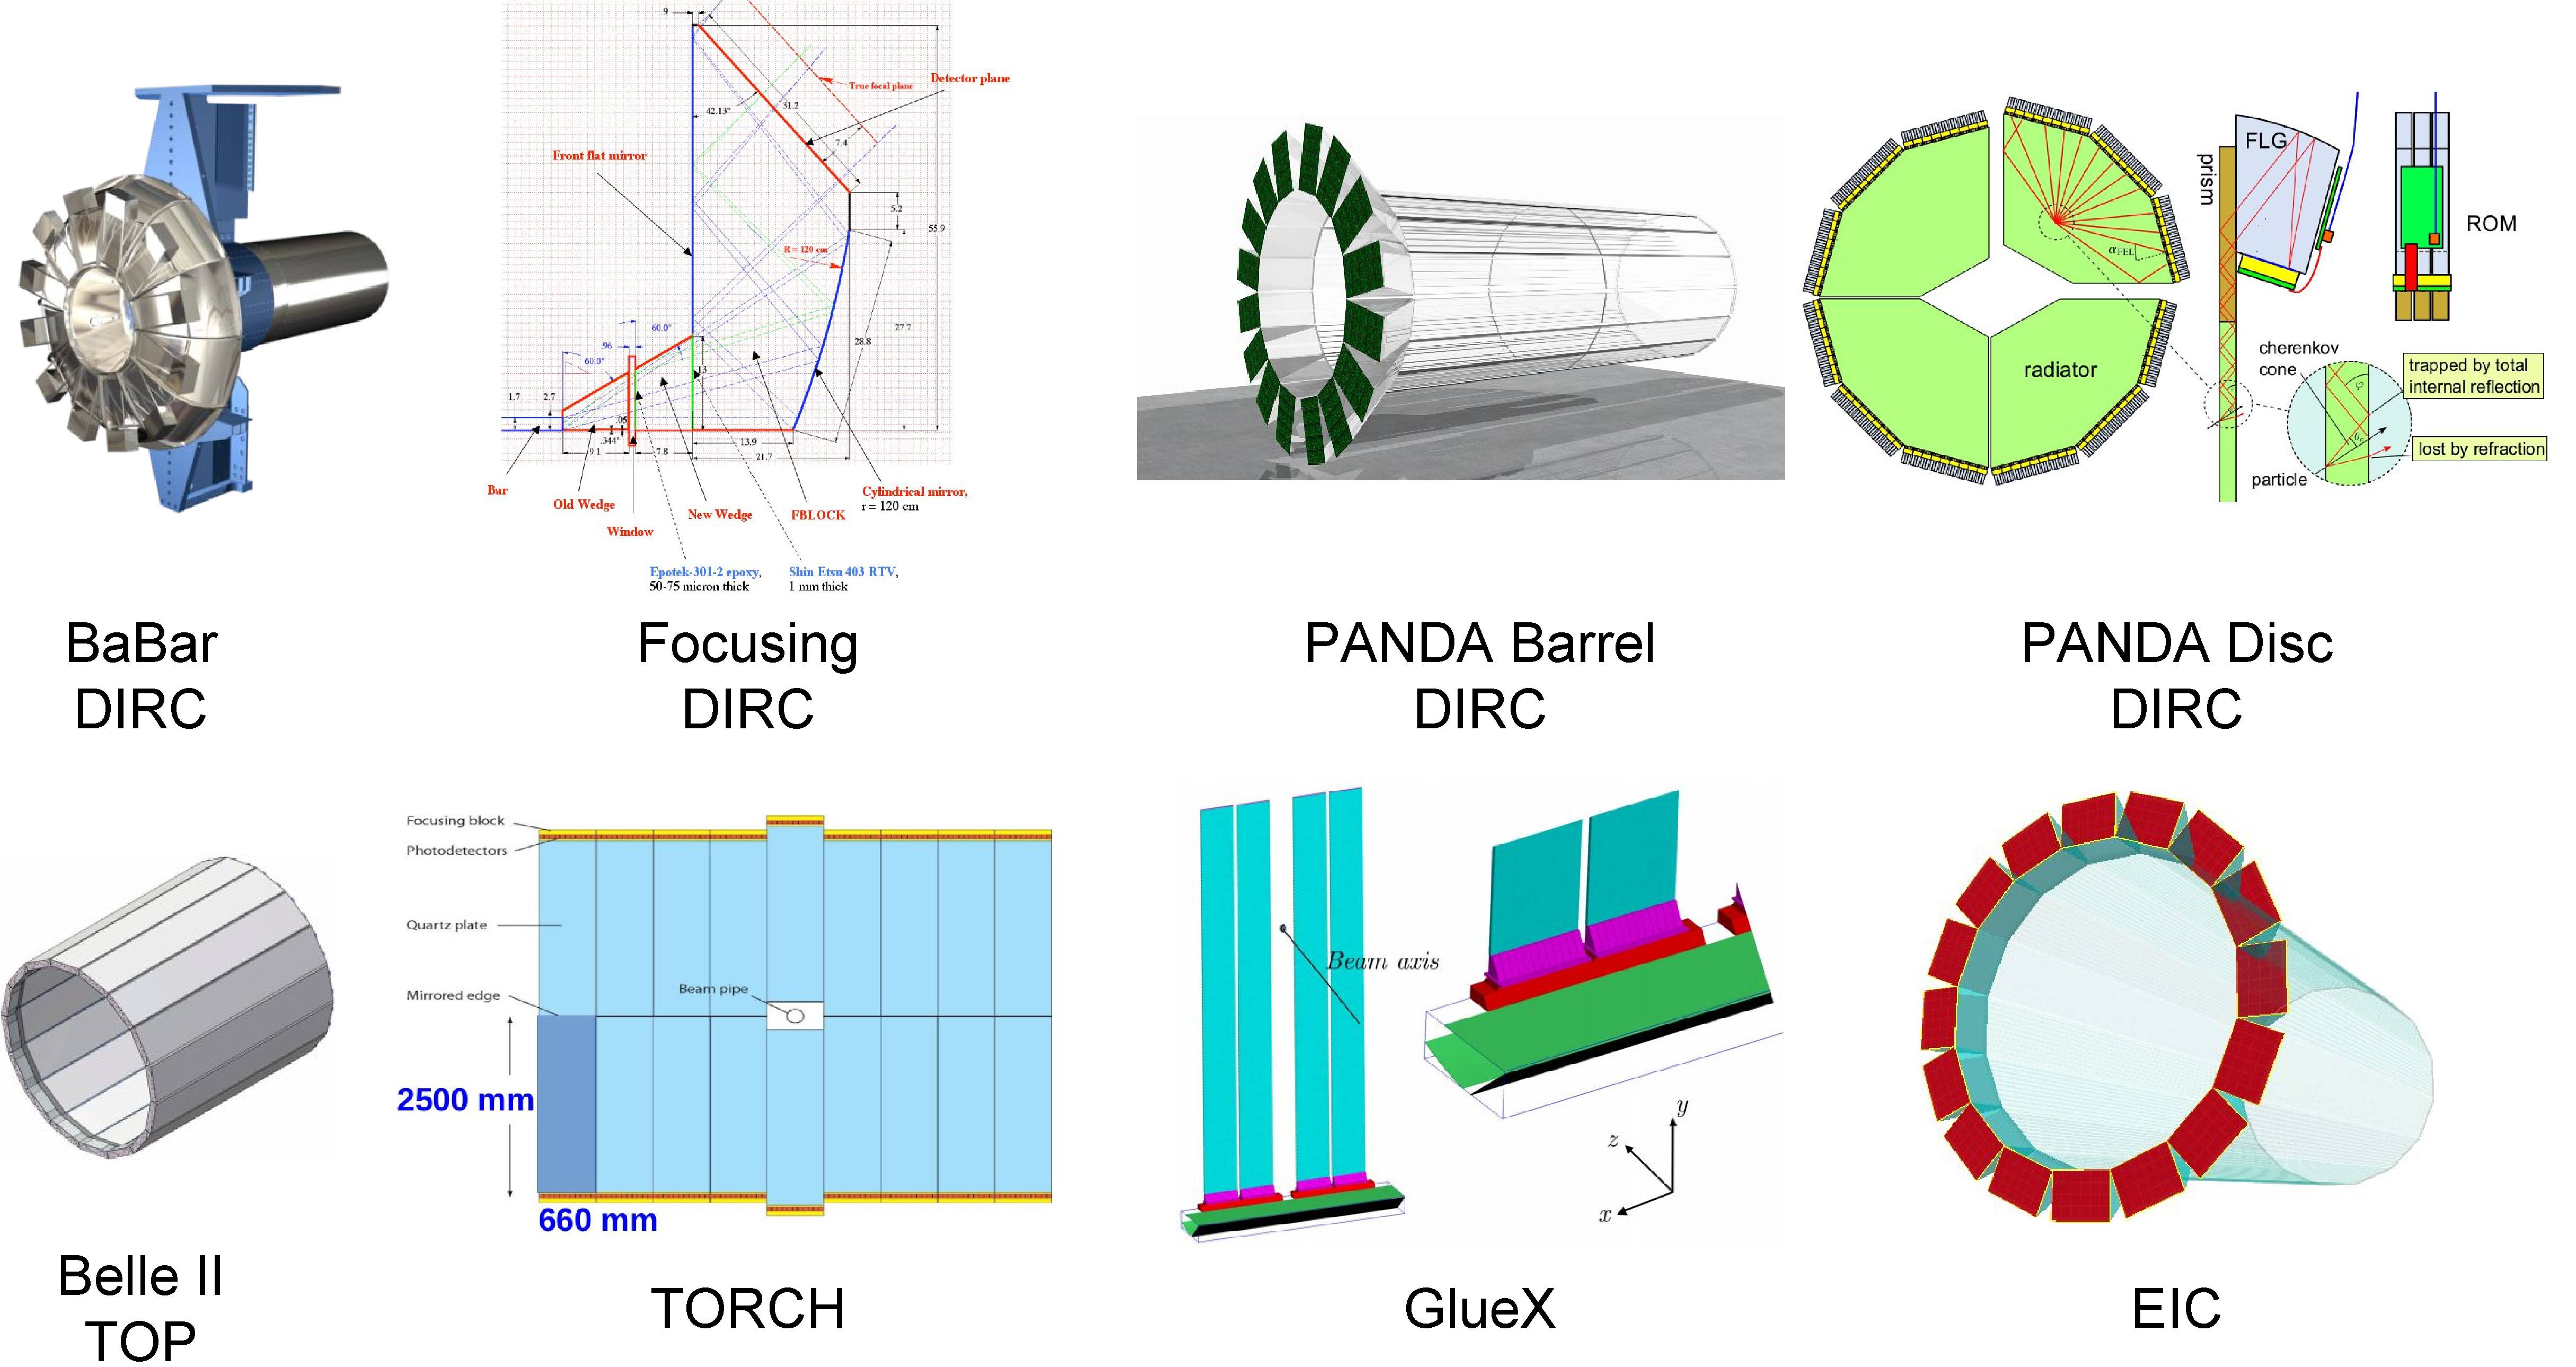
\includegraphics[width=\textwidth]{dirc_evolution.pdf}
	\caption{Evolution of the DIRC concept. From top left to bottom right: BaBar Barrel DIRC, Focusing DIRC, PANDA Barrel DIRC, PANDA Disc DIRC, Belle II Time of Propagation DIRC, LHCb TORCH DIRC, GlueX DIRC, EIC DIRC}
	\label{fig:dirc_evolution}
\end{figure}

%----------------------------------------------------------------------
%	RECONSTRUCTION SECTION
%----------------------------------------------------------------------
\section{Hit Patterns and Particle Separation Methods}
As mentioned previously, a DIRC detector is a compact RICH system that relies on internal reflection of the Cherenkov photons in the radiating material. However, as is illustrated in Figure \ref{fig:dircbasics}, not all of the light produced inside the radiator is internally reflected as photons with an angle less than the critical angle (approximately $43^{\circ}$ for the interface from fused silica to air) with respect to the surface will escape the radiator. Because of this loss of photons the hit patter of a DIRC is only roughly half of a typical RICH ring, which is then mirrored depending on where the photon exited the radiator. If the expansion volume is more radially compact the two ring segments become stacked side by side. To complicate matters further, if the expansion volume is small enough that reflections from the sides occur then the ring segments are folded on top of themselves to create much more complicated hit patterns. Figure \ref{fig:ring_comparison2} illustrates this folding of the hit pattern due to expansion volume size. Figure \ref{fig:prism_reflections} shows the contribution to the folded pattern from single reflections inside a prism shaped expansion volume.

Two approaches were used in the analysis presented in this thesis for particle species separation: reconstruction of the Cherenkov angle using a geometrical reconstruction method similar to the one used by the BaBar DIRC, and time-based imaging using probability density functions (PDFs) \footnote{In this manuscript, 'PDF' refers to a 'probability distribution function' and does NOT refer to either an Adobe(TM) Portable Document Format or to a parton distribution function.} similar to that used by the Belle II Time of Propagation counter.

\begin{figure}[H]
	\centering
	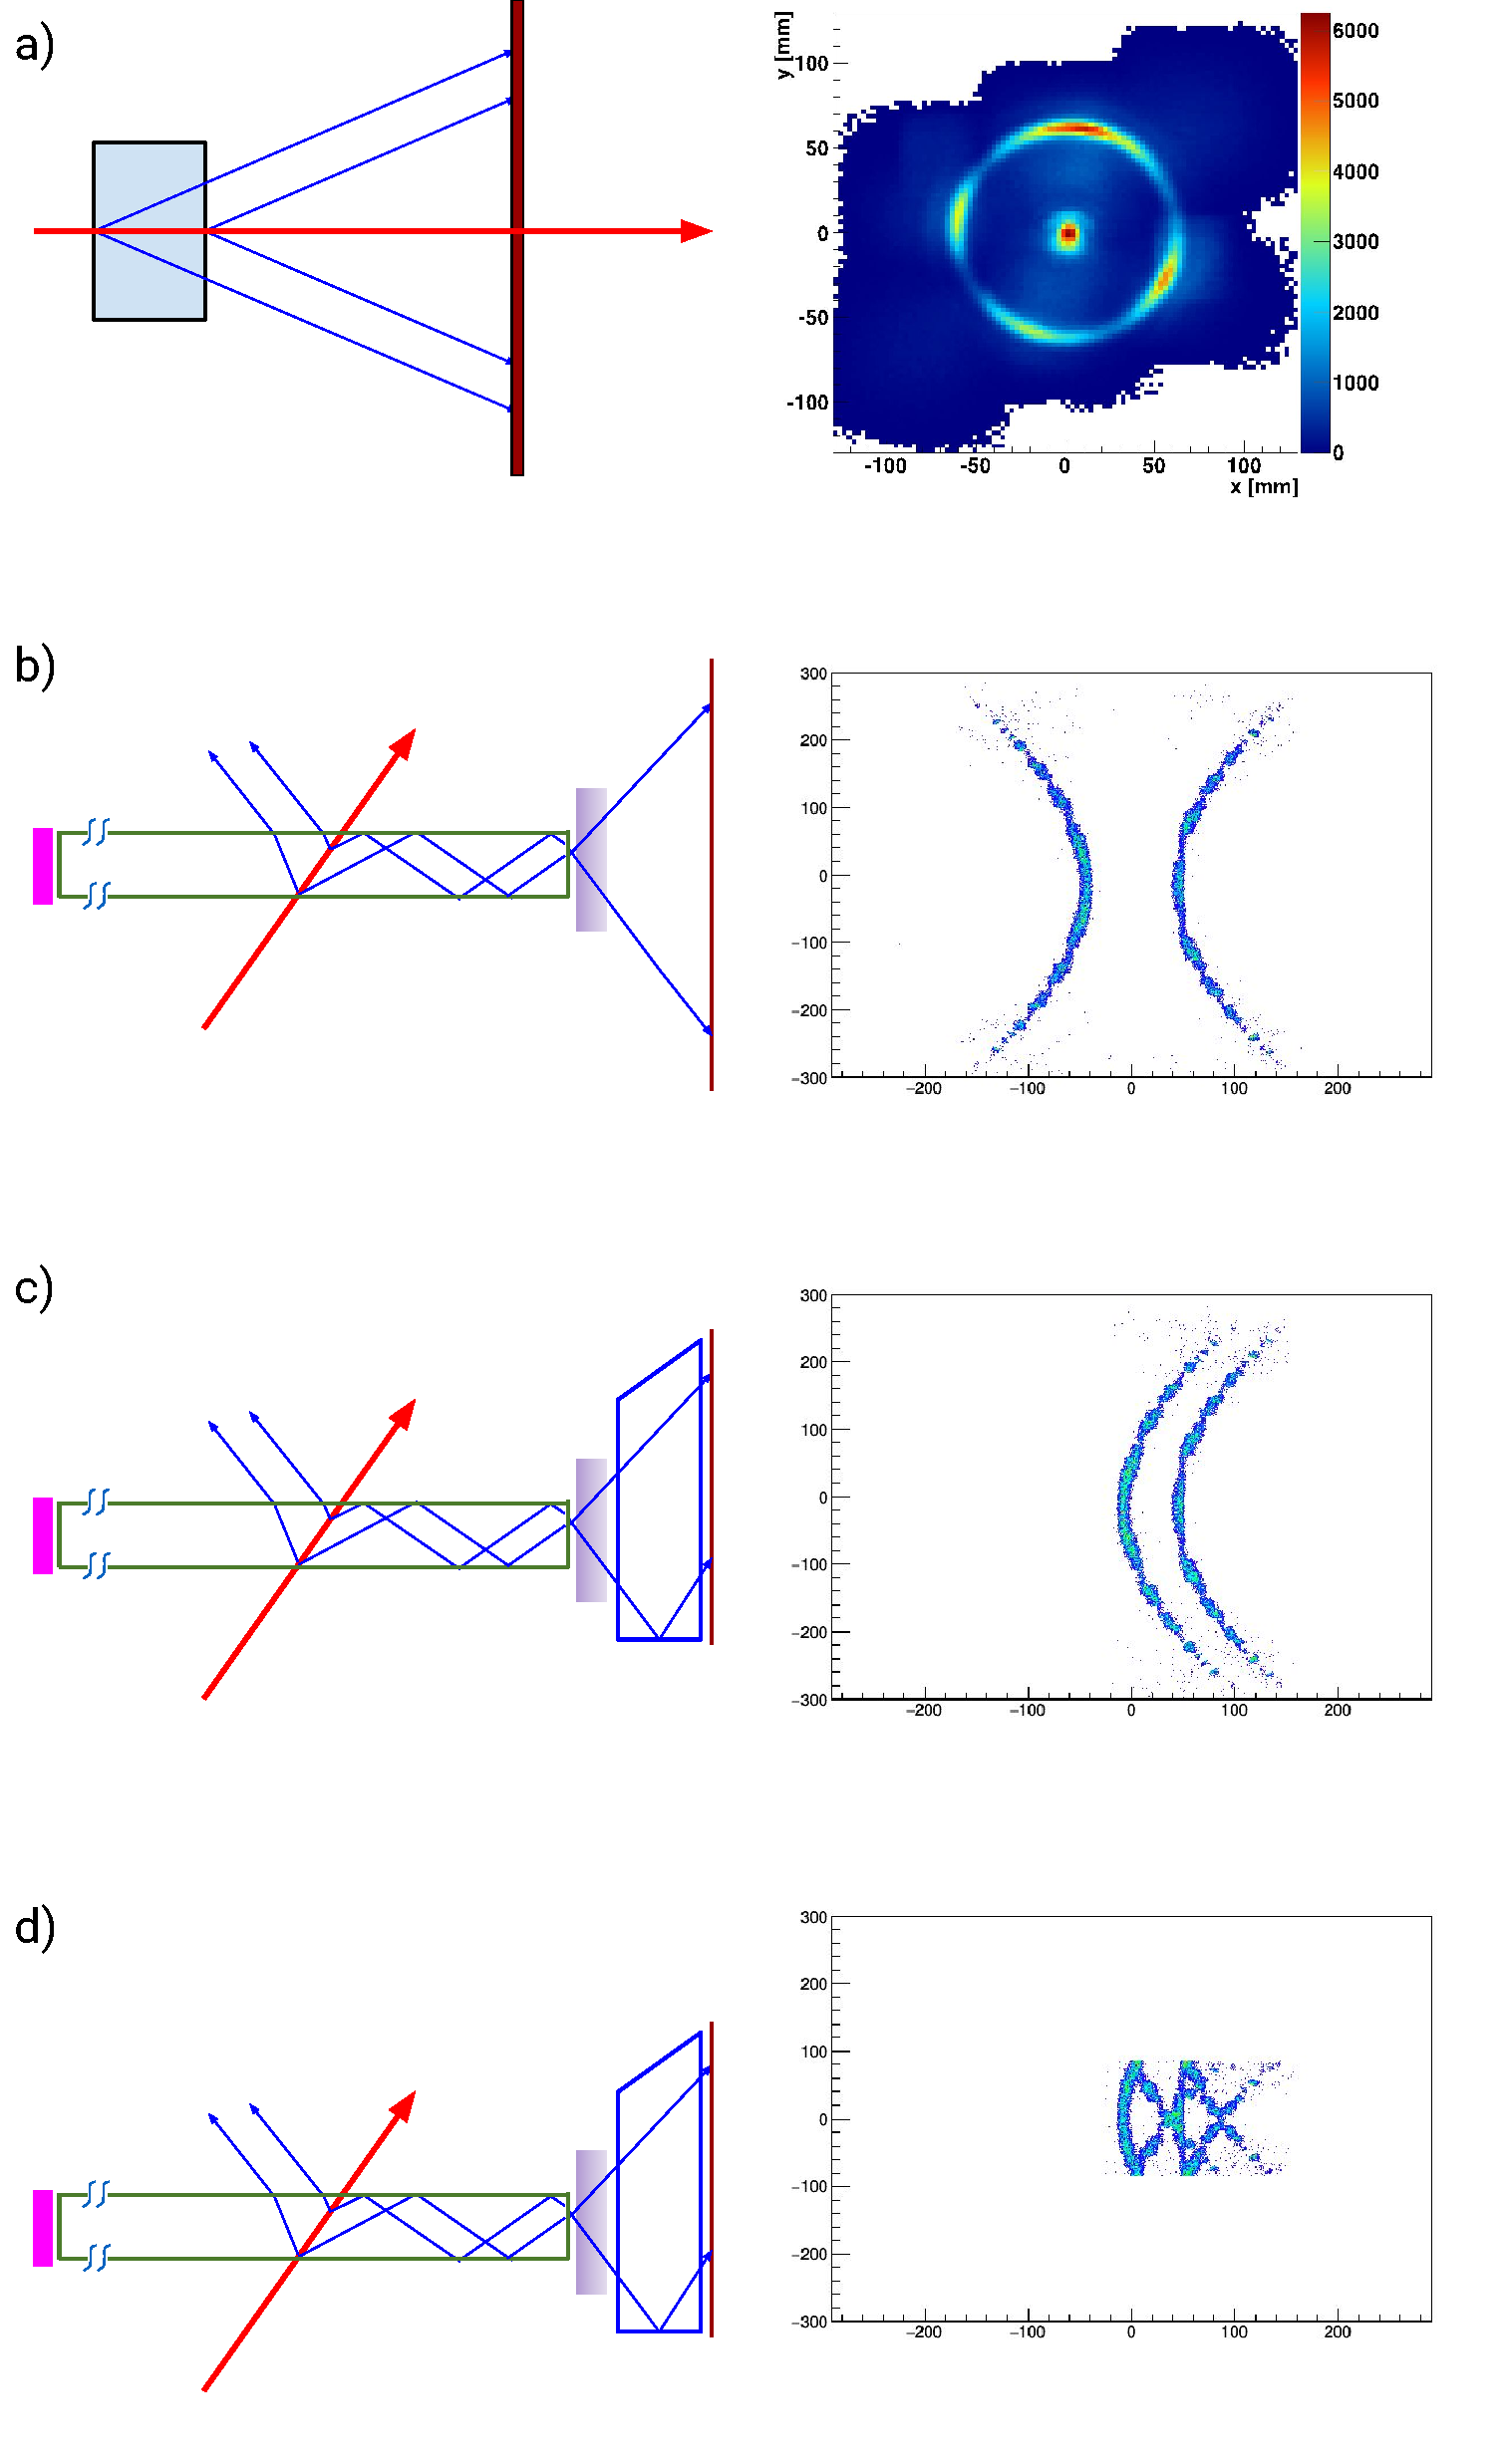
\includegraphics[scale=0.43]{ring_comparison2.pdf}
	\caption{Various detector geometries (left) and the resulting simulated hit patterns (right) from 1000 identical particles. A typical RICH detector (a), produces a very nice ring pattern. A DIRC detector with a sufficiently large expansion volume using a thin radiator bar (b) produces two ring segments. A DIRC with a radially compact expansion volume (c) will reflect one of the ring segments so that it will stack side by side. Finally, a DIRC detector with a compact expansion volume both radially and transversely (i.e. into and out of the page) (d) will cause the ring segments to fold in on themselves, making a fish-like pattern. The DIRC patterns are viewed from the back of the detector plane and rotated $90^{\circ}$ clockwise relative to the corresponding geometry.}
	\label{fig:ring_comparison2}
\end{figure}


\begin{figure}[H]
	\centering
	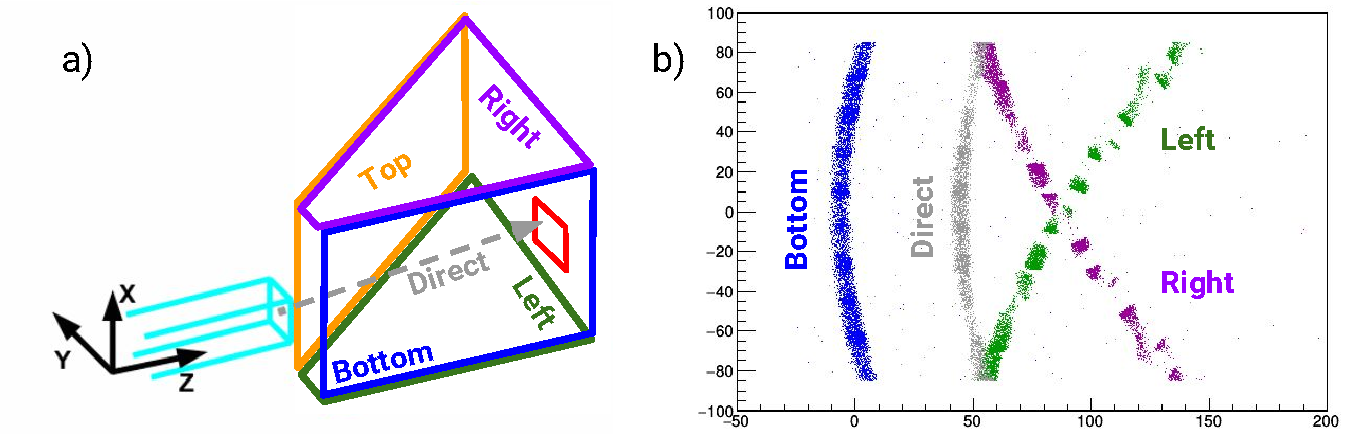
\includegraphics[width=\textwidth]{prism_reflections.pdf}
	\caption{For a prism-shaped expansion volume (a) different segments of the hit pattern correspond to different paths taken (b). Paths with multiple reflections inside the prism (e.g. bottom-left) have been excluded for simplicity.}
	\label{fig:prism_reflections}
\end{figure}

\subsection{Cherenkov Angle Reconstruction}
The emmission angle between a single photon and the particle track can be reconstructed from the observed photon coordinates on the detector plane. The spacial position of the centers of the radiator bar and the struck pixel are known and used to define the 3-dimensional direction vector $\vec{k} = (k_x, k_y, k_z)$ pointing from the center of the bar end to the center of the pixel (shown in Figure \ref{fig:k_vector}) . The $k$-vector is defined as the photon exit vector just inside the bar. The direction vector from the bar center to the pixel center along with Snell's law are used to determine the $k$-vector. Excluding aberrations, any photon reaching this pixel originated with the same direction vector at the end of the bar, regardless of the photon origination point. Together with the particle direction $\vec{p} = (p_x, p_y, p_z)$ the Cherenkov angle for each photon can be calculated from

\begin{equation}
	\thetaC = \arccos\left(\frac{\vec{k}\times\vec{p}}{|p|}\right)
\end{equation}

\begin{figure}[!htb]
	\centering
	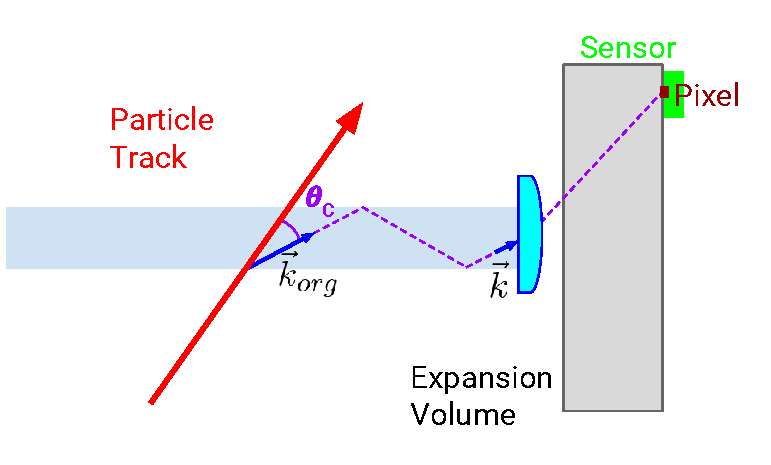
\includegraphics[width=0.65\textwidth]{k_vector.pdf}
	\caption{Schematic of the geometric reconstruction concept, with a photon (purple) being emitted from the particle track. The direction of the k-vector can be used to determine the original direction vector, $\vec{k}_{org}$, of the photon and is used for the reconstruction of $\thetaC$.}
	\label{fig:k_vector}
\end{figure}

In order to get a value of the k-vector for each pixel a photon gun is used in Geant4 to illuminate the detector plane. Roughly $10^5$ photons are created at the end of the bar uniformly and allowed to propagate through the expansion volume and onto the photosensors. The initial value of the k-vector, the propagation time,  number of bounces inside the expansion volume, and sensor and pixel number are all stored in a large table, called a lookup table (LUT). The values in the LUT are independent of particle species and momentum and only depends upon the detector geometry (e.g. the focusing optic, or the location of the bar relative to the expansion volume). Because of this a LUT for a given geometry can be generated before taking data. Another advantage to the geometrical reconstruction is that a full simulation of the particle track is not needed which saves a lot of computation, as much of the computing power used during a simulation is used for the photon propagation through the bar.

Unfortunately, the direction of the k-vector as reconstructed by the pixel does not uniquely define the directionality of $\vec{k}_{org}$. Because the number of reflections inside the bar cannot be known there are 8 possibilities, or ambiguities, for the original directionality of the photon that must be considered (forward/backward, up/down, and left/right). Figure \ref{fig:bar_ambiguities} illustrates a 2D simplification of this problem, showing 4 possible photon directions propagating from the particle track. Here each of $\theta_{1-4}$ are possible values for the true Cherenkov angle. In the full 3D space this leads to up to 8 possibilities to be considered for the k-vector for each detected photon, and therefore up to 8 values of the Cherenkov angle $\thetaC$.

\begin{figure}[!htb]
	\centering
	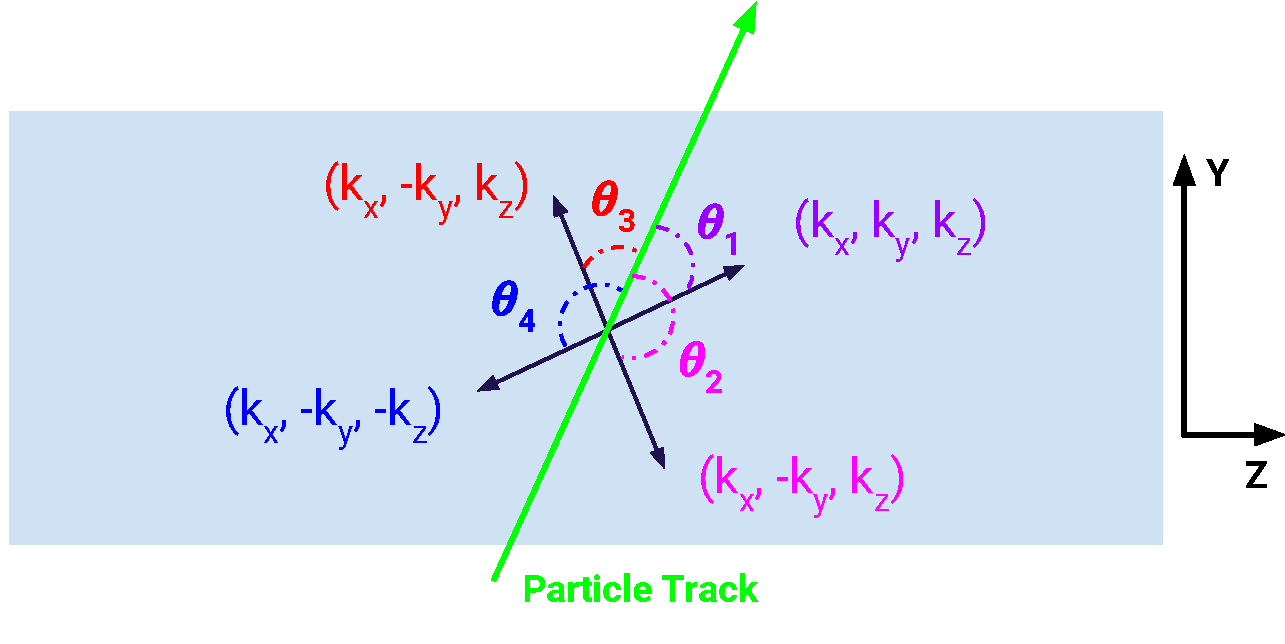
\includegraphics[width=0.7\textwidth]{bar_ambiguities.pdf}
	\caption{2D illustration showing all possible combinations of k-vector directions off of the particle track. Not shown are the additional 4 components where $k_x \rightarrow -k_x$.}
	\label{fig:bar_ambiguities}
\end{figure}

In addition to ambiguities coming from guessing the initial directionality of the k-vector inside the bar there are also ambiguities coming from the multiple possible paths that a photon could take from the center of the bar to a pixel inside the expansion volume. Figure \ref{fig:prism_ambiguities} shows a prism-shaped expansion volume, similar to that used in the analysis presented later in Chapter \ref{ch:analysis}, showing the labeling of the surfaces and an example of ambiguous photon paths from the bar to a pixel on the detector plane.

The number of ambiguous paths that are reconstructed can be reduced by averaging the initial direction of all photons in the LUT that have the same number and types of reflections and land in the same pixel. As a simplified example, see Figure \ref{fig:lut_averaging}

\begin{figure}[!htb]
	\centering
	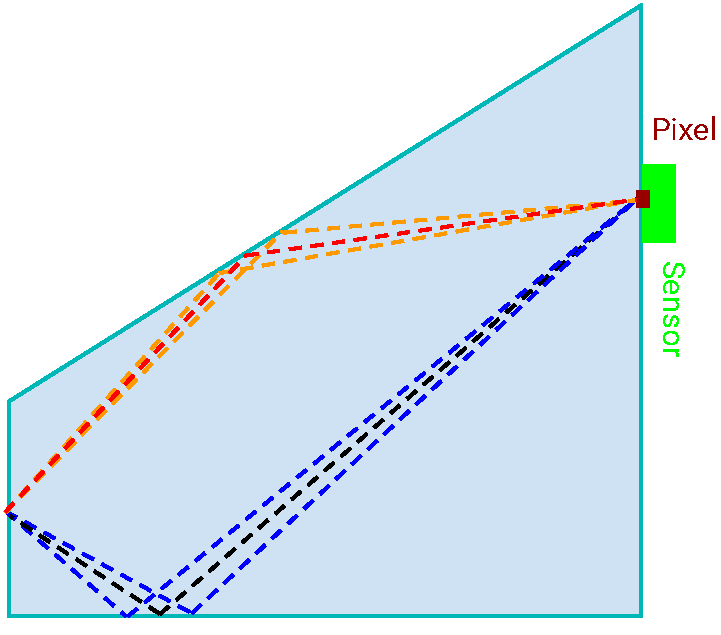
\includegraphics[width=0.75\textwidth]{lut_averaging.pdf}
	\caption{2D example of averaging LUT entries to reduce prism ambiguity reconstructions. The two photons reflecting off of the bottom prism face (blue) have been averaged to the one black photon. The two photons reflecting off of the top prism face (orange) have been average to the red photon. In this simplified example the number of entries in the LUT have been reduced by half. Angles have been exaggerated.}
	\label{fig:lut_averaging}
\end{figure}

The Cherenkov angle is not, however, only reconstructed for one photon, but for up to 160 photons per particle track. For each photon at least one of these reconstructed $\thetaC$ values is correct, while the others contribute to a combinatorial background in a spectrum of the reconstructed angle, an example of which can be seen in Figure \ref{fig:combinatorial_background} for 7 GeV/c protons with a $125^{\circ}$ polar angle and made with an averaged path LUT.

\begin{figure}[!htb]
	\centering
	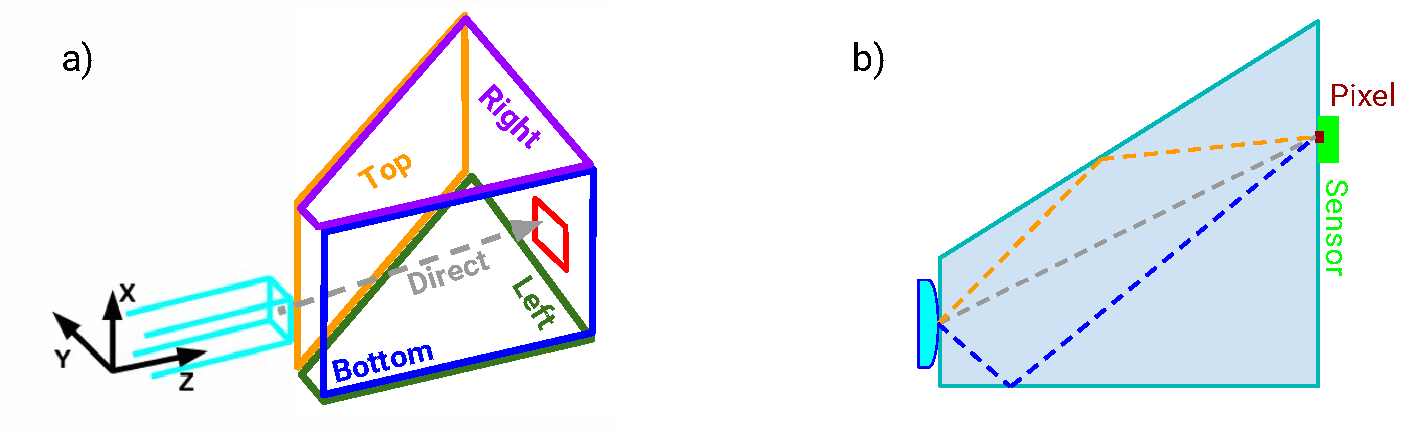
\includegraphics[width=\textwidth]{prism_ambiguities.pdf}
	\caption{Illustration of possible ambiguities in the $\thetaC$ reconstruction coming from possible paths in a prism-shaped expansion volume. Each face is labeled in a) along with an example of a direct path, while b) shows 3 possible paths that lead from the bar to a certain pixel: 1 top reflection (gold), 1 bottom reflection (blue), and 1 direct path (gray).}
	\label{fig:prism_ambiguities}
\end{figure}

\begin{figure}[!htb]
	\centering
	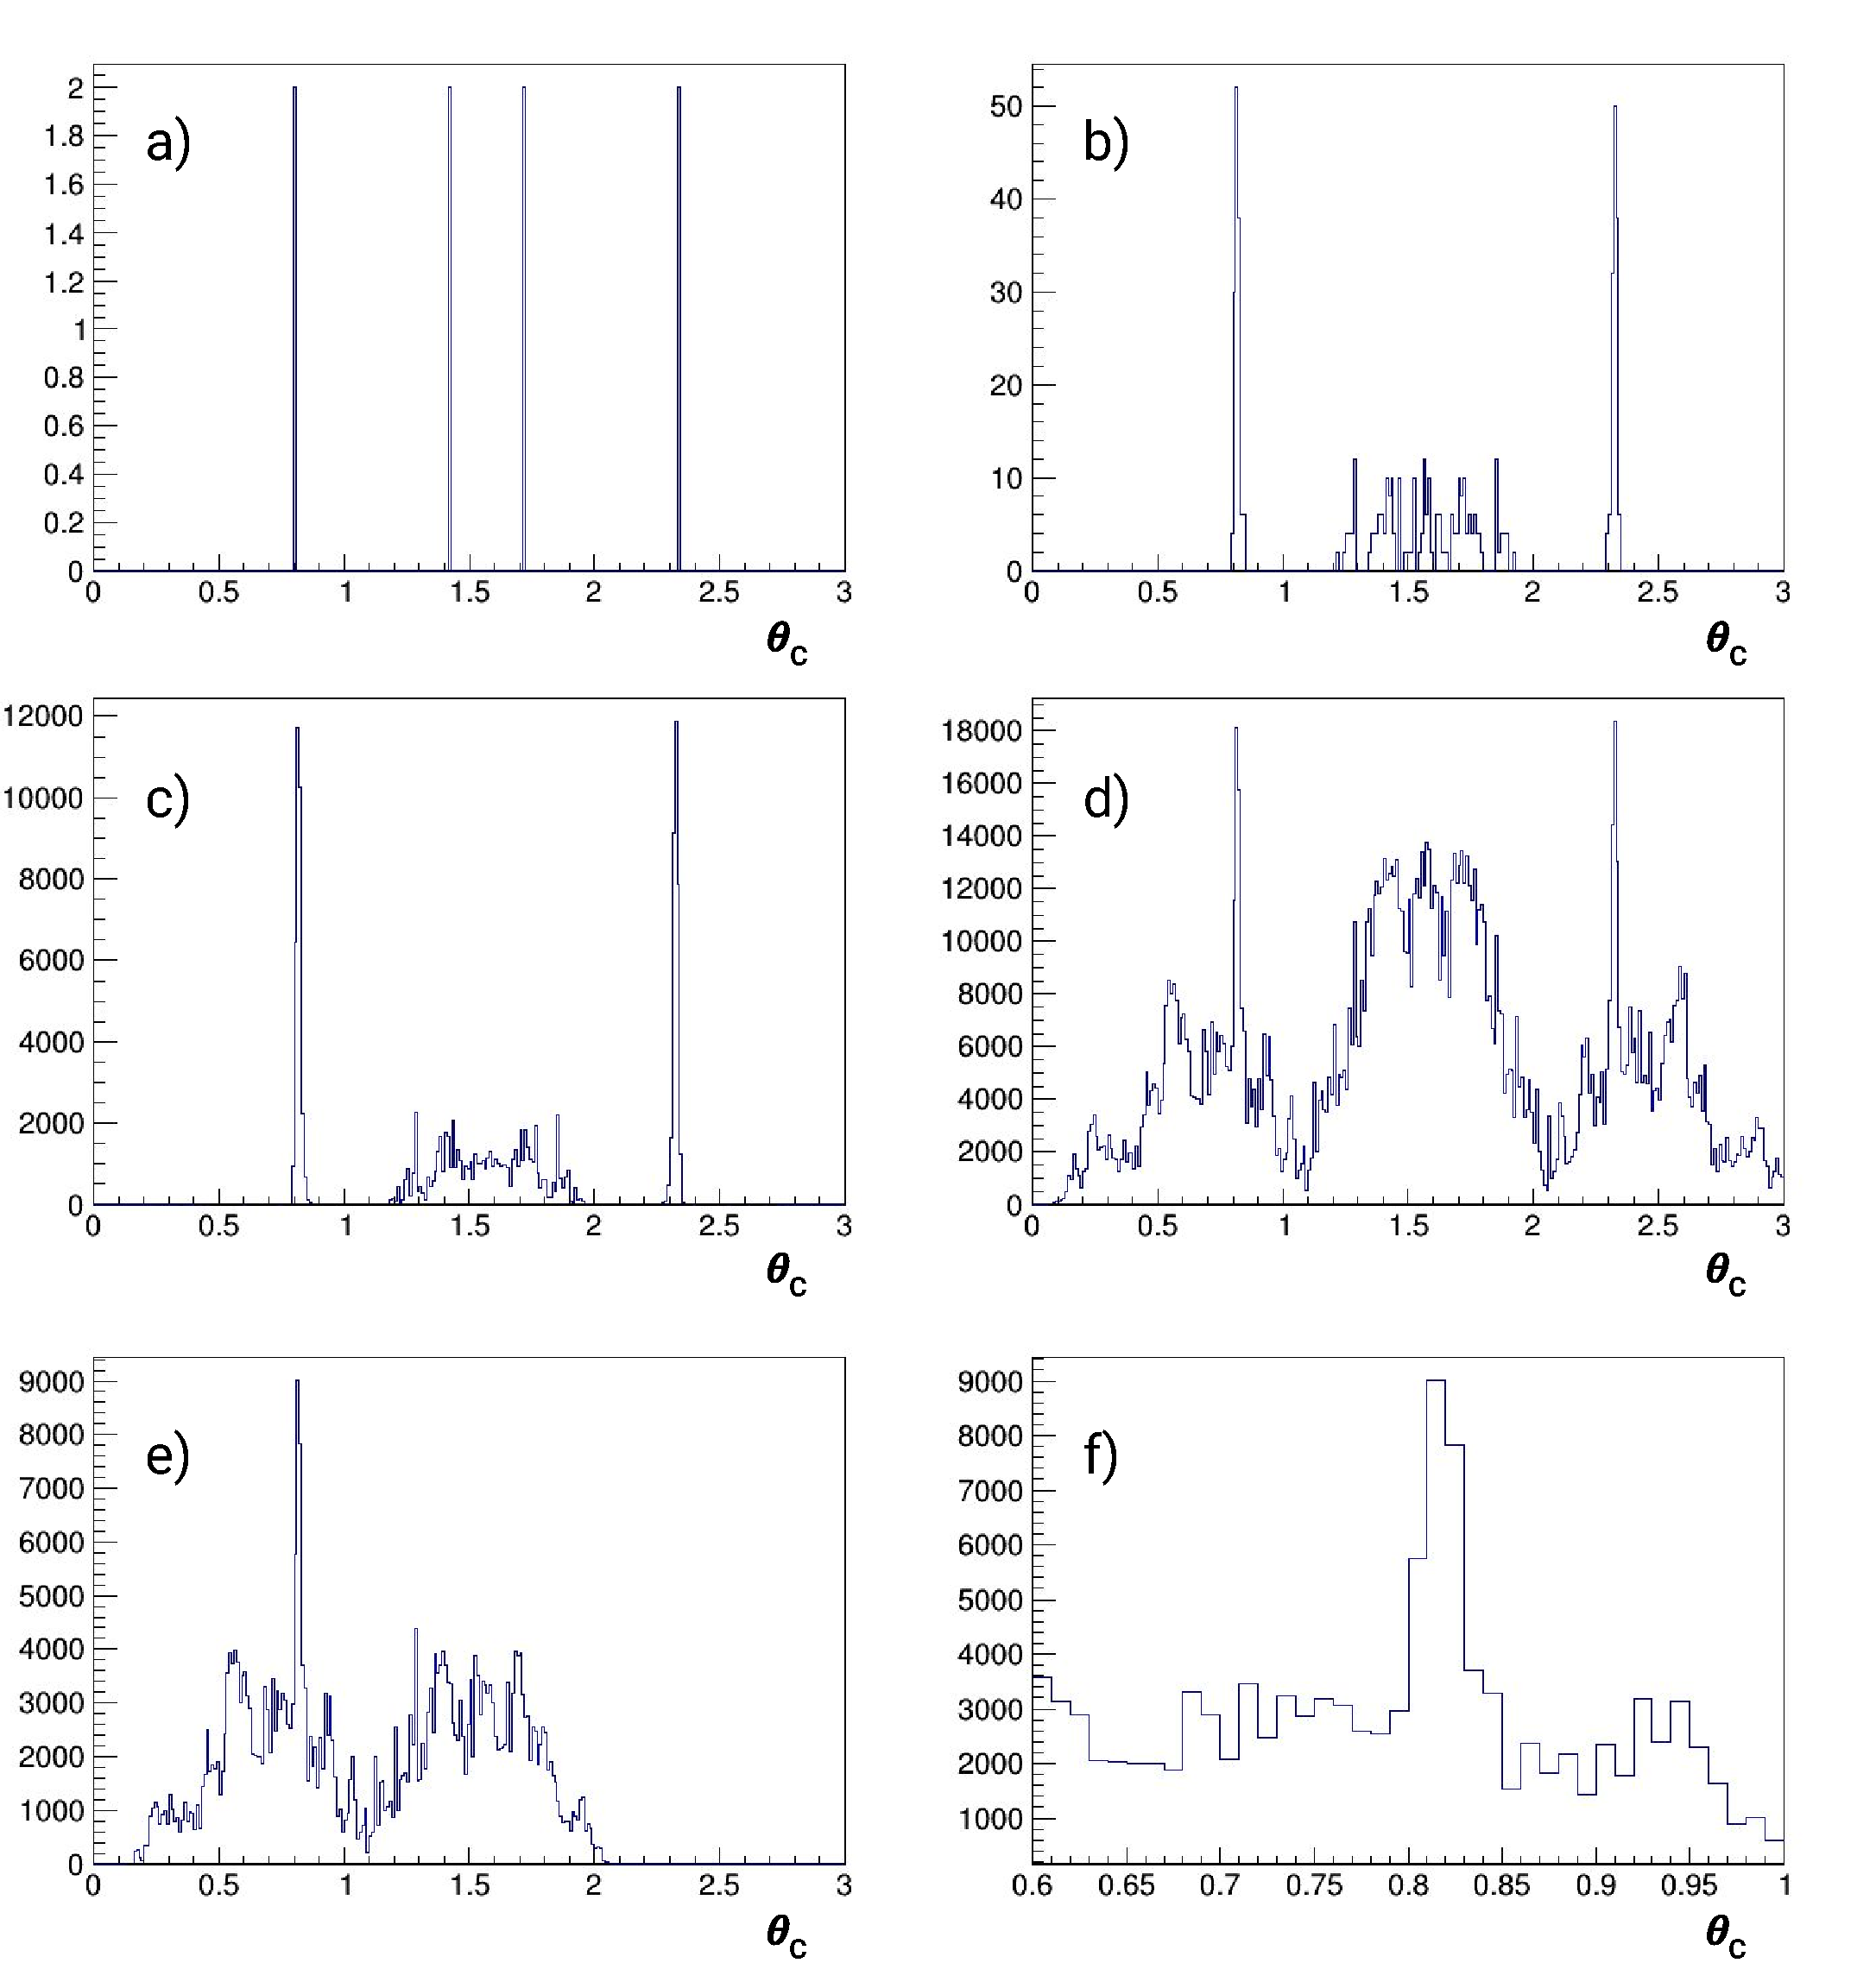
\includegraphics[width=\textwidth]{combinatorial_background.pdf}
	\caption{Simulated reconstructed Cherenkov angle per photon from a 7 GeV/c particle with a polar angle of $125^{\circ}$ for: a) one photon from a proton with only bar ambiguities, b) all photons from one proton with only bar ambiguities, c) all photons from 1000 identical protons with only bar ambiguities, d) all photons from 1000 identical protons with both bar and prism ambiguities, e) same as d) but with constraints on the photon angle with the bar surface and neglecting y direction flips due to zero beam divergence, and f) a zoom showing a buildup around the calculated value of 816 mrad along with a combinatorial background.}
	\label{fig:combinatorial_background}
\end{figure}

\subsection{Time-Based Imaging}
The other method of particle species separation that can be used for a DIRC is time-based imaging or time-based reconstruction, similar to that used by the Belle II Time-Of-Propagation counter. To do time-based reconstruction one must first generate a PDF of the timing information of each detector pixel for each value of particle species, momentum, polar track angle, and detector geometry (e.g. lens and bar types), thus giving a 5-dimensional function  of the timing distribution of photon hits \cite{PANDA_barrel}. Currently these PDFs cannot be computed analytically, so they are constructed computationally by either taking actual test beam data, or running simulations with sufficient statistics such that each pixel that can have a hit with the configuration of interest has a large enough occupancy to produce a more or less smooth PDF.

To reconstruct a data or simulation file using these PDFs the photon arrival time for each pixel with a recorded hit is compared to the PDF for each particle species, and the time-based likelihood of that hit corresponding to a given particle species $X$ is calculated as $L_{X} = \ln(h_{X})$, where $h$ is the value of the PDF for the given hit time. One can then do a pair-wise difference of these likelihood values (e.g. $L = L_{p} - L_{\pi}$) to build a log-likelihood distribution between two particle hypotheses and extract a separation power for particle identification. The separation power for time-based reconstruction between two particle species is given by the magnitude of the difference of the two log likelihood plots divided by the average sigma. An example of time-based reconstruction for a bar radiator with a prism expansion volume is shown in Figure \ref{fig:time-based_reco} for pions and kaons in a plate radiator with a prism expansion volume.

This method of particle separation is also very useful for plate-type radiators as the LUTs in the geometric reconstruction assume the photons come from the center of the bar, which is no longer a good assumption for wide plates. 

\begin{figure}[!htb]
	\centering
	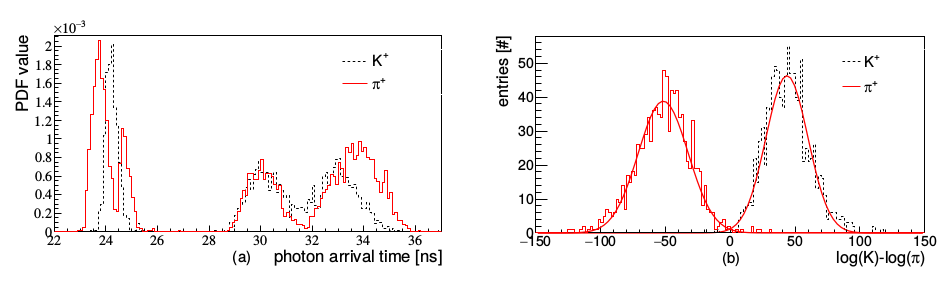
\includegraphics[width=\textwidth]{time-based_reconstruction.png}
	\caption{An example of time-based reconstruction for a plate radiator with a prism expansion volume for kaons (dashed) and pions (red). Photon arrival times for one MCP-PMT pixel are shown in a), and b) is the log-likelihood difference for kaon and pion hypotheses for multiple 3.5 GeV/c particles at $22^\circ$ polar angle \cite{PANDA_barrel}.}
	\label{fig:time-based_reco}
\end{figure}